\section{Testing: Neutron Criticality} \label{section diffusion}
As a simple yet sufficiently complex problem to test stochastic collocation for uncertainty quantification, we make use of a 2-dimensional quarter-core reactor neutron diffusion code, which makes use of two energy groups and 11 distinct regions to nonlinearly solve for the $k$-eigenvalue of the system using Jacobian-free Newton-Krylov mothods.  The sample model uses five materials and, without introducting uncertainty, is nearly exactly critical.

\subsection{Problem Description}
This test code solves the following equation:
\begin{equation}
-\nabla D_g\nabla\phi_g+\Sigma_{a,g}\phi_g=\sum_{g'}\Sigma_s^{g'g}\phi_{g'}+\frac{\chi_g}{k}\sum_{g'}\nu\Sigma_{f,g'}\phi_{g'}, \hspace{15pt}g\in(1,2),
\end{equation}
where $k$ is the $k_\text{eff}$ eigenvalue, $g$ denotes an energy group ($g$=1 is high energy, $g$=2 is low energy), $\Sigma_s^{g'g}$ is the macroscopic scattering cross section from group $g'$ into group $g$, and $\chi_g$ is the group-based neutron fission emission spectrum.  For this particlar problem, we consider no upscattering and all fissions in to the high energy group.
The two-dimensional core is shown in Fig. \ref{coremap} and the material properties are listed in Table \ref{tab:coremats}.
\begin{figure}[h]
\centering
   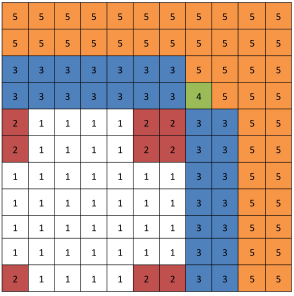
\includegraphics[width=0.4\textwidth]{./graphics/core}
   \caption{Core Map}
   \label{coremap}
\end{figure}
\begin{table}[h]
\centering
\begin{tabular}{c c | c c c c}
Region & Group & $D_g$ & $\Sigma_{a,g}$ & $\nu\Sigma_{f,g}$ & $\Sigma_{1,2}$ \\ \hline
1 & 1 & 1.255 & 8.252e-3 & 4.602e-3 & 2.533e-2 \\
 & 2 & 2.11e-1 & 1.003e-1 & 1.091e-1 & \\ \hline
2 & 1 & 1.268 & 7.181e-3 & 4.609e-3 & 2.767e-2 \\
 & 2 & 1.902e-1 & 7.047e-2 & 8.675e-2 & \\ \hline
3 & 1 & 1.259 & 8.002e-3 & 4.663e-3 & 2.617e-2 \\
 & 2 & 2.091e-1 & 8.344e-2 & 1.021e-1 & \\ \hline
4 & 1 & 1.259 & 8.002e-3 & 4.663e-3 & 2.617e-2 \\
 & 2 & 2.091e-1 & 7.3324e-2 & 1.021e-1 & \\ \hline
5 & 1 & 1.257 & 6.034e-4 & 0 & 4.754e-2 \\
 & 2 & 1.592e-1 & 1.911e-2 & 0 & 
\end{tabular}
\caption{Basic Material Properties for Core}
\label{tab:coremats}
\end{table}

\subsubsection{Base Results}
Without introducing uncertainty, the flux profiles by group are shown in Figs. \ref{figg1} and \ref{figg2} and $k-$effective is unity to 6 significant digits.  Using 100 cells (10 by 10) in each region shown in Fig. \ref{coremap}, $k$ is 1.000048123 converged to 8 orders of magnitude.
\begin{figure}[h]
\centering
  \begin{subfigure}[b]{0.45 \textwidth}
   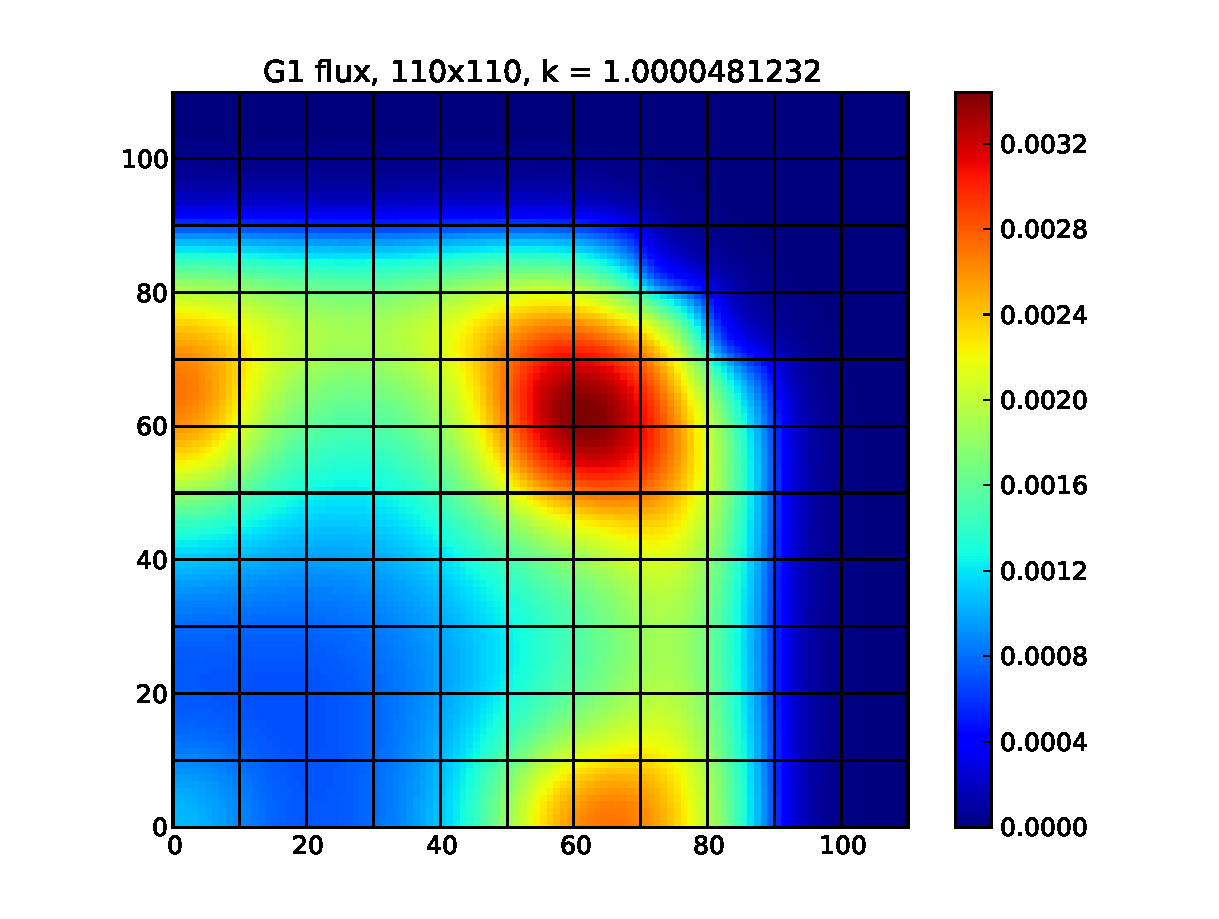
\includegraphics[width=\textwidth]{./graphics/g1_50_flux}
   \caption{High Energy}
   \label{figg1}
  \end{subfigure}
  \begin{subfigure}[b]{0.45\textwidth}
   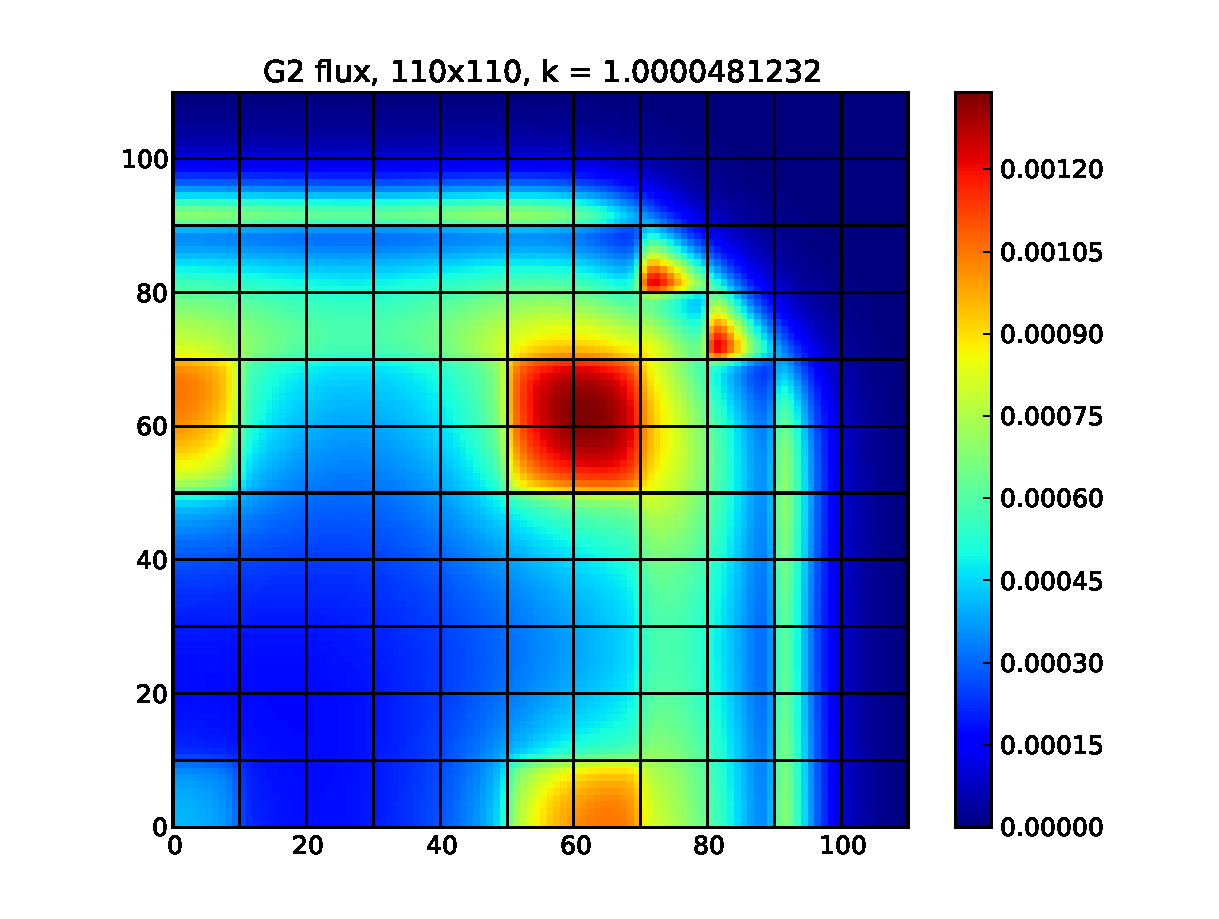
\includegraphics[width=\textwidth]{./graphics/g2_50_flux}
   \caption{Low Energy}
   \label{figg2}
  \end{subfigure}
\caption{Base Flux Profiles for Core (no uncertainty)}
\end{figure}

\subsection{Single Variable Uncertainty}
We begin by introducing uncertainty into a single material property; in this case, we chose the Material 1 low-energy absorption cross section.  We test both the uniform uncertainty distribution and normal distribution.   In both cases, the mean value is $\Sigma_a^2=0.1003 \text{ cm}^{-1}$.

For the uniform distribution, we allow the value to range uniformly from 30\% above to 30\% below the mean value, or $\Sigma_a^2\in(0.07021,0.13039)$ (this leads to $k\in(0.9707,1.276)$).  The coefficients for the standard orthonormal Legendre expansion are given as follows for several expansion orders, to 4 significant figures:
\begin{table}[h!]
\centering
\begin{tabular}{c || c c c c}
Coeff & 2 & 4 & 6 & 8\\ \hline
$f_0$ & 1.479 & 1.476 & 1.469 & 1.476 \\
$f_1$ & -9.698e-2 & -1.075e-1 & -1.109e-1 & -1.081e-1 \\
$f_2$ &  & 5.223e-2 & 5.946e-2 &  5.282e-2\\
$f_3$ &  & -1.471e-2 & -6.970e-3 &  -1.275e-2\\
$f_4$ &  &  & -5.973e-3 &  -2.302e-3\\
$f_5$ &  &  & -4.862e-3 &  2.285e-3\\
$f_6$ &  &  &  &  6.144e-4\\
$f_7$ &  &  &  &  1.245e-3
\end{tabular}
\caption{Uniform Uncertainty Expansion Coefficients for Diffusion}
\end{table}

Similar to the uniform distribution, for the normal distribution we assign a standard deviation of 1\% of the mean.  The coefficients from the standard orthonormal Hermite expansion are given as follows for expansion orders, to 4 significant figures:
\begin{table}[h!]
\centering
\begin{tabular}{c || c c c c}
Coeff & 2 & 4 & 6 & 8\\ \hline
$f_0$ & 1.353 & 1.338 & 1.321 & 1.351 \\
$f_1$ & -4.319e-2 & -5.928e-2 & -6.903e-2 & -5.051e-2 \\
$f_2$ &  & 3.083e-2 & 4.056e-2 & 2.728e-2 \\
$f_3$ &  & -2.640e-4 & 1.144e-2 & -8.195e-3 \\
$f_4$ &  &  & -6.678e-3 & -1.524e-3 \\
$f_5$ &  &  & -1.656e-2 & 2.150e-3 \\
$f_6$ &  &  &  & 5.933e-4 \\
$f_7$ &  &  &  & -1.584e-3 
\end{tabular}
\caption{Uniform Uncertainty Expansion Coefficients for Diffusion}
\end{table}

To demonstrate the use of the reduced-order models (ROMs) generated by the code, we sampled each expansion with a million Monte Carlo samples of the uncertain variable.  We performed this in both single-processor and embarassingly parallel cases; the run time for an eigth-order expansion was 52 seconds in 4-processor parallel and 195 seconds on a single processor, both for the uniform uncertainty case.  The values were then collected in 100 evenly-distributed bins across the range of the values obtained and collected as a numeric PDF.  The results for both the uniform uncertainty and normal uncertainty are shown in Figs. \ref{diff_unipdfs} and \ref{diff_normpdfs}.


\begin{figure}[h!]
\centering
%  \begin{subfigure}[b]{0.45 \textwidth}
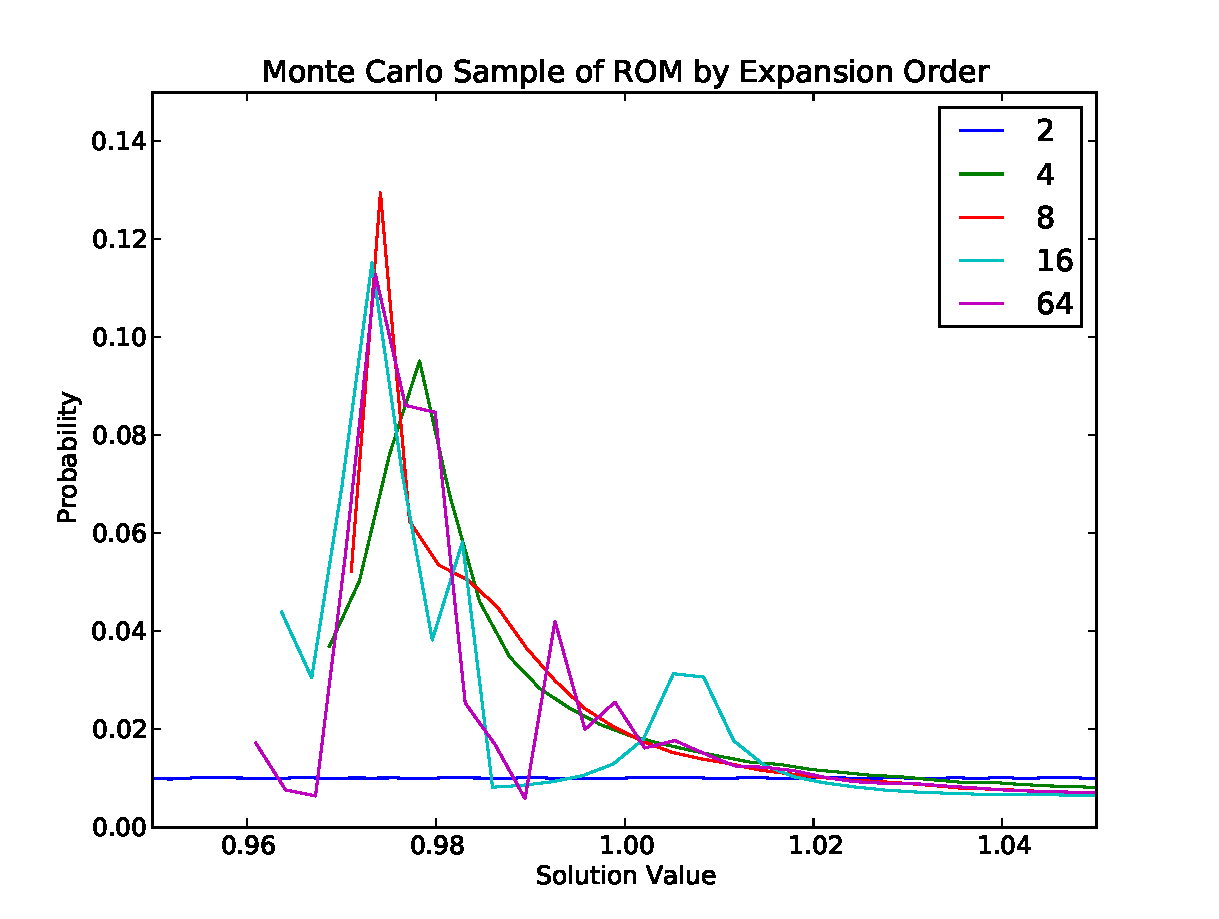
\includegraphics[width=0.7\linewidth]{./graphics/diff_romsample}
\caption{Uniform uncertainty}
\label{diff_unipdfs}
%  \end{subfigure}
\end{figure}
\begin{figure}
\centering
%  \begin{subfigure}[b]{0.45\textwidth}
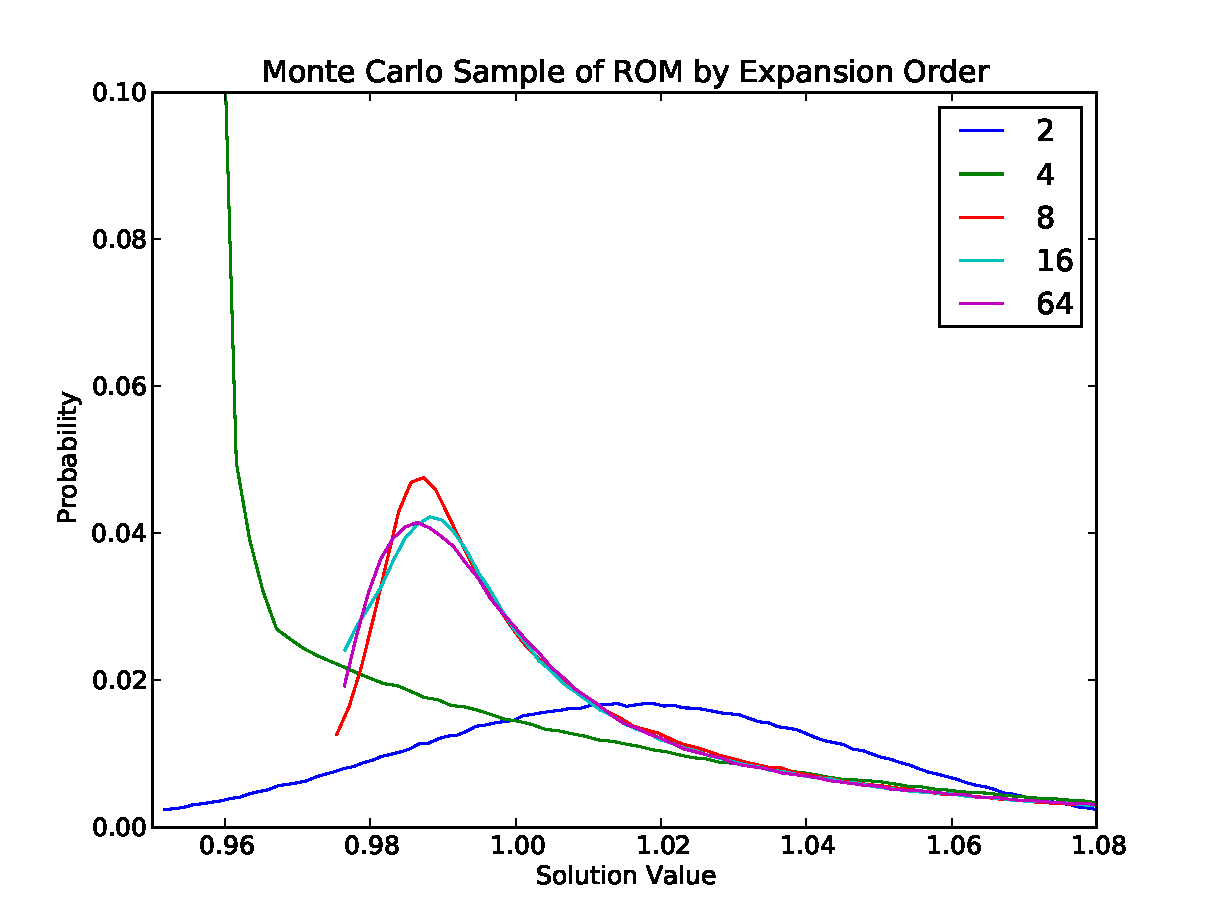
\includegraphics[width=0.7\linewidth]{./graphics/diff_normrom}
\caption{Normal uncertainty}
\label{diff_normpdfs}
%  \end{subfigure}
 % \caption{PDFs of expansion ROMs}
\end{figure}